% !TEX root = ./Basilisk-avsLibrary20170812.tex




\section{Library Description}
The AVS lab has released a set of astrodynamics C-functions\footnote{\url{http://hanspeterschaub.info/AVS-Code.html}} that facilitate common orbital or rotational dynamics evaluations.  The functions are openly available, and are included with the AIAA Education Series textbook \emph{Analytical Mechanics of Space Systems}\cite{schaub} since the first release in 2003.  The most up to date public versions are found on the AVS web page.

\subsection{{\tt linearAlgebra} Library}
The linear algebra library provides numerous C-based functions to perform basic matrix math operations.  For a complete list of functions supported, consult the {\tt linearAlgebra.h} file.   The library provides common matrix and vector manipulation tools such as performing a matrix product, including the transpose operators, as well as doing the matrix inverse operations.  The vector library supports doing dot and cross product operations, as well as taking a norm of a vector.  Helper functions are provided to initial zero or identity matrices, as well as check if the matrix elements are zero





\subsection{{\tt rigidBodyKinematics} Library}
The rigid body kinematics library provides a range of functions related to mapping between attitude coordinates descriptions, compute the addition or subtraction of orientations, as well as returning the differential kinematic equations.  This library has been included with Reference~\citenum{schaub} since 2003 and has been used extensively across a range of research projects.  Reference~\citenum{schaub} provides all the mathematical details of the transformation used here in Chapter 3, while Appendix E provides a comprehensive discussion of all the algorithms included.



\subsection{{\tt orbitalMotion} Library}
Common celestial mechanics tools are implemented in the {\tt orbitalMotion} library, including transforming between anomaly angles, converting between inertial Cartesian position and velocity vector components and classical orbit elements, as well as evaluating simple space environment parameters.  The following developments use the notation and formulation of Chapter 9 in Reference~\citenum{schaub}.  The variable naming is reflected within the software code.


\subsubsection{Classical Orbital Elements}
The classical orbit elements are given by
$$
	(a, e, i, \Omega, \omega, f)
$$
where $a$ is the semi-major axis or SMA, $e$ is the eccentricity, and $(\Omega, i, \omega)$ are the 3-1-3 Euler angles called the right ascension of the ascending node, inclination, and argument of periapsis, respectively. These are illustrated in Figure~\ref{fig:orbit313}. Inclination satisfies $0\leq i\leq\pi$. For nonparabolic motion the semi-latus rectum $p$ is
\begin{equation}
	p = a (1-e^{2})
\end{equation}
\begin{figure}[t]
	\centering
	\subfigure[Orbit Frame Orientation Illustration]
	{\label{fig:orbit313}
	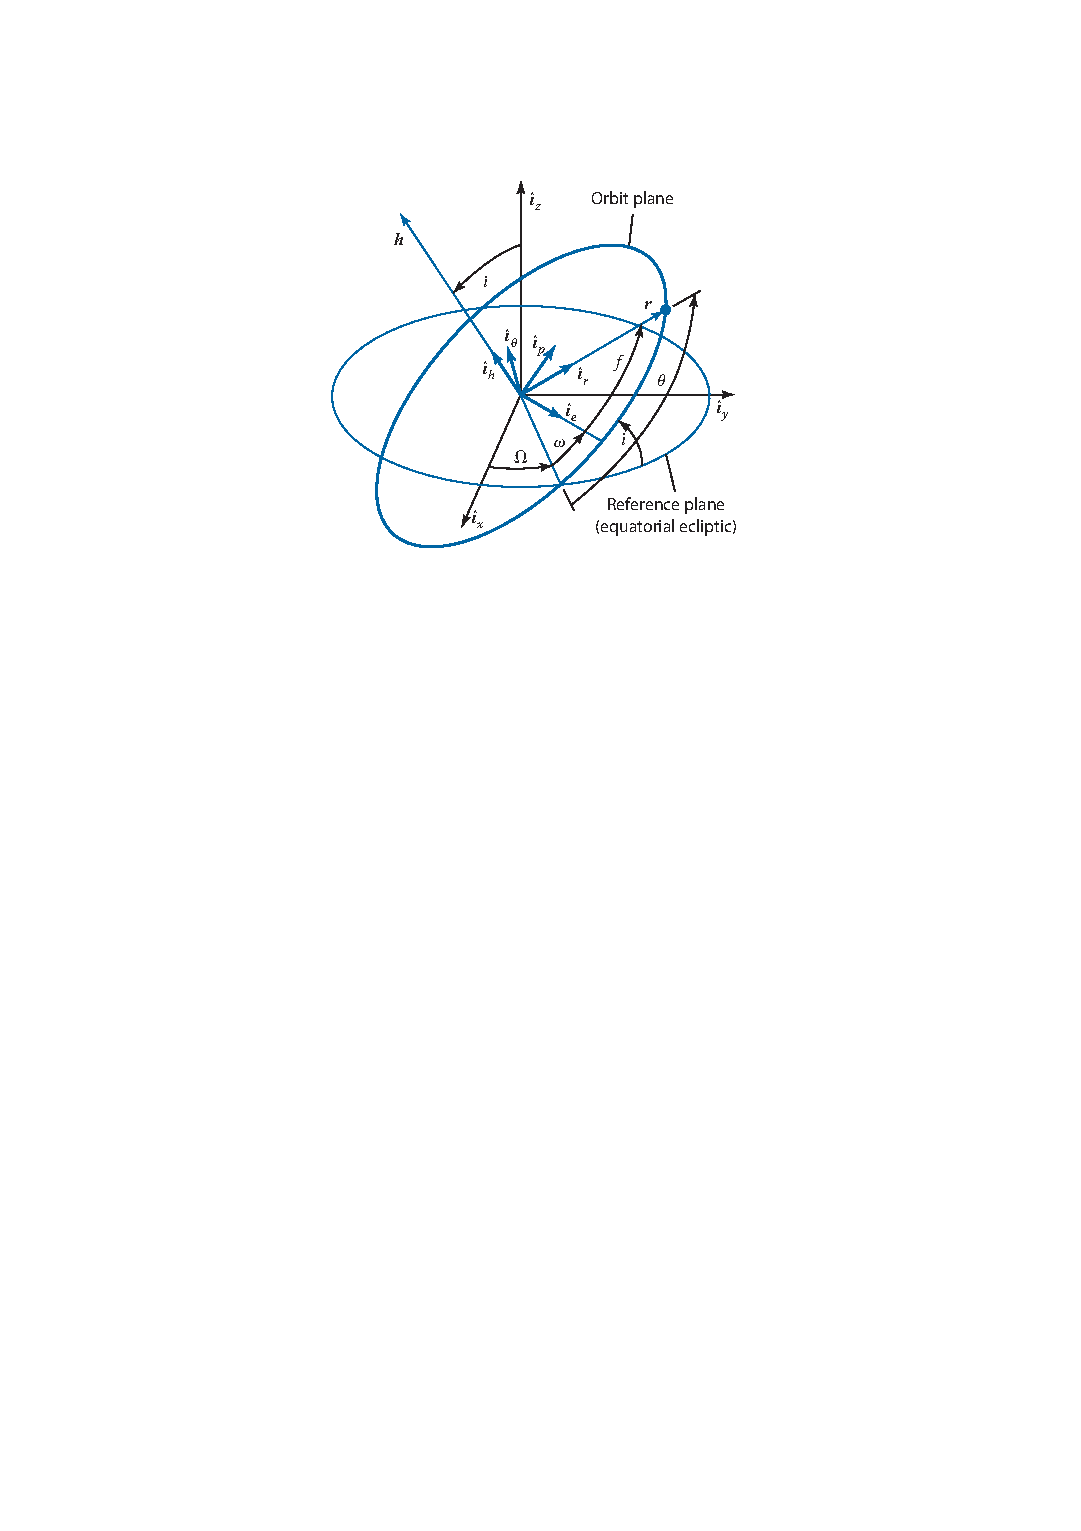
\includegraphics[width=0.45\textwidth]{Figures/orbit313}}
	\\
	\subfigure[Classical orbital parameter Illustration for an Elliptic Orbit]
	{\label{fig:orbitElliptic}
	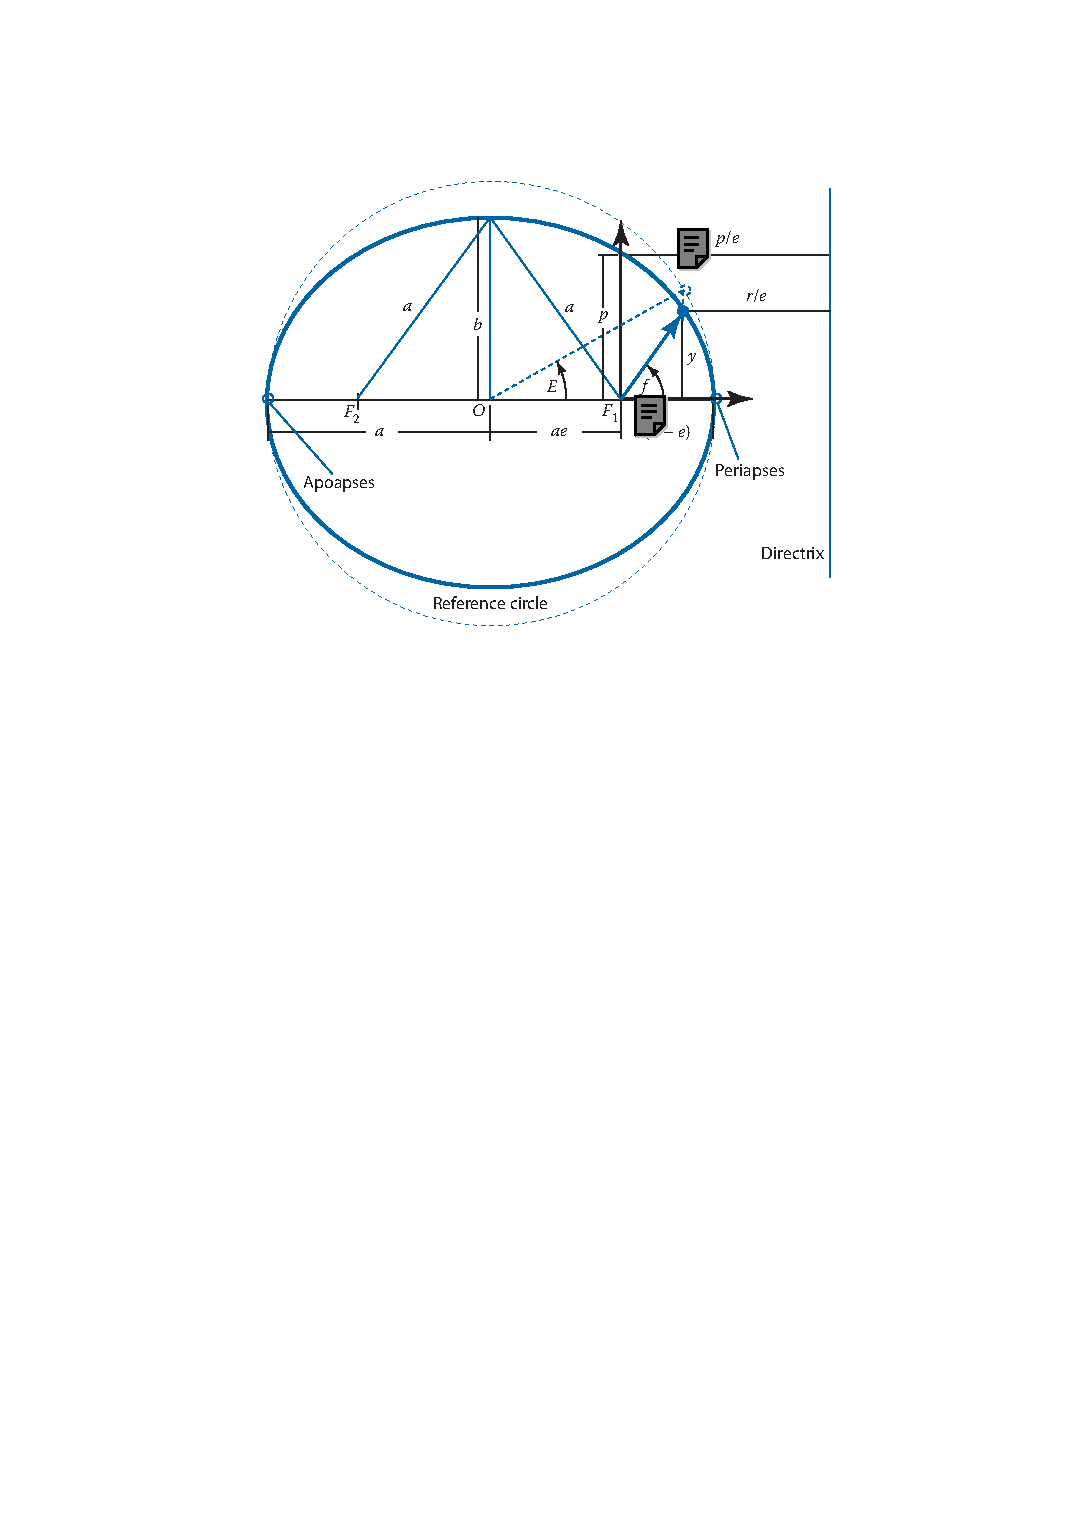
\includegraphics[width=0.45\textwidth]{Figures/orbitEllipse}}
	\subfigure[Classical orbital parameter Illustration for a Hyperbolic Orbit]
	{\label{fig:orbitHyperbolic}
	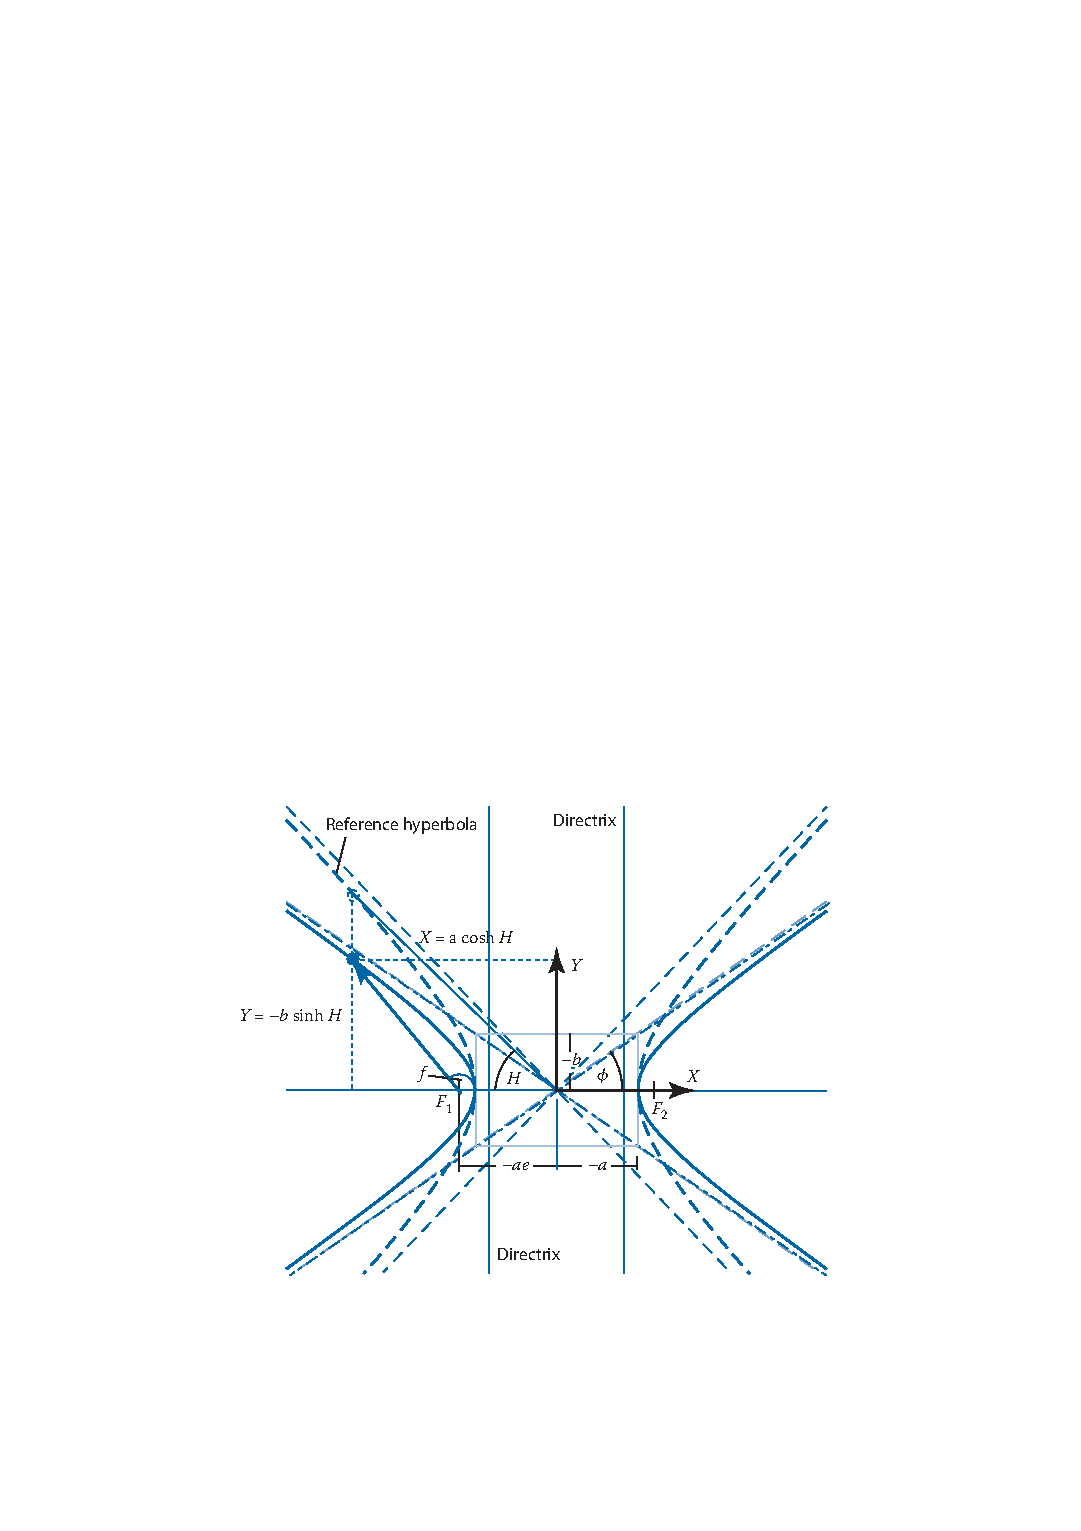
\includegraphics[width=0.45\textwidth]{Figures/orbitHyperbola}}
	\caption{Orbit Elements, Axes and Frames Illustrations.\cite{schaub}}
	\label{fig:orbitParameters}
\end{figure}

Finally, the true anomaly angle is given by $f$, while the eccentric anomaly angle is expressed through $E$ as illustrated in Figure~\ref{fig:orbitElliptic} for an elliptic orbit scenario.  The true and eccentric anomaly are related through\cite{schaub}
\begin{equation}
	\tan\left( \frac{f}{2} \right) = \sqrt{ \frac{1+e}{1-e} } \tan\left( \frac{E}{2} \right)
\end{equation}
The mean anomaly angle $M$ relates to the eccentric anomaly angle $E$ through\cite{schaub}
\begin{equation}
	M = E - e \sin E
\end{equation}

The classical orbit elements for a hyperbolic scenario are shown in Figure~\ref{fig:orbitHyperbolic}. The SMA is negative for a hyperbolic orbit. For nonrectilinear motion, the true anomaly $f$ measures position from periapsis. Rectilinear motion instead uses an energy-dependent anomaly convention described below. The hyperbolic anomaly $H$ relates to $f$ through
\begin{equation}
	\tan\left( \frac{f}{2} \right) = \sqrt{ \frac{e+1}{e-1}} \tanh\left( \frac{H}{2} \right)
\end{equation}
The hyperbolic mean anomaly is defined in terms of the hyperbolic anomaly through
\begin{equation}
	N = e \sinh H - H
\end{equation}


The inverse mean-anomaly mappings solve Kepler's equation with bracketed Newton iteration, using bisection whenever a Newton step leaves the bracket. Stable residual and derivative expressions reduce cancellation near unit eccentricity and avoid overflow for large hyperbolic anomalies. Iteration stops when the correction is at most $4\epsilon$ times the magnitude of the current anomaly, or when the next representable iterate is unchanged; $\epsilon$ is double-precision machine epsilon. The limit is 200 iterations. Invalid inputs or exhausted iteration produce a diagnostic and NaN in C, or an exception in Python. Elliptic results retain whole revolutions, subject to the resolution of the input and output angles.




\subsubsection{Orbit Element to Cartesian Coordinate Conversions}
Let $\leftexp{N}{\bm r}_{C/N}$ and $\leftexp{N}{\bm v}_{C/N}$ be the inertial spacecraft center of mass $C$ position and velocity vector matrix representations, expressed with respect to inertial frame \frameDefinition{N} components.  Functions are provided to map from classical orbit elements to these Cartesian coordinates through {\tt elem2rv()}, as well as the inverse mapping from Cartesian to classical orbit elements through {\tt rv2elem()}.

\paragraph{{\tt elem2rv()} Function}
The general conversion of classical orbit elements to inertial Cartesian components is outlined in section 9.6.2 of Reference~\citenum{schaub}. For nonrectilinear motion, the orbit radius at true anomaly $f$ is
\begin{equation}
	r = \frac{p}{1 + e \cos f}
\end{equation}
If the satellite is not on a parabola, then $p$ is computed using
\begin{equation}
	p = a(1-e^{2})
\end{equation}
For a nonrectilinear parabola, the core C and Python conversions use the sentinel $a=0$, $e=1$, and
\begin{equation}
	p = 2r_{p}
\end{equation}
where $r_{p}>0$ is supplied in {\tt rPeriap}. Eccentricity $e=1$ alone does not identify a parabola, because rectilinear motion also has unit eccentricity. Distances must use the same unit L as the gravitational parameter $\mu$ in L$^3$/s$^2$; angles are in radians. Open-conic anomalies must satisfy $|f|<\arccos(-1/e)$ after reduction to the principal interval. Collisions and anomalies at or beyond infinity are rejected. Trigonometric evaluation retains the phase of large wrapped inputs without division by a rounded $2\pi$.

The true latitude angle $\theta$ is given by
\begin{equation}
	\theta = \omega + f
\end{equation}
The inertial position vector is then given by\cite{schaub}
\begin{equation}
\bm r_{C/N} =r {\begin{matrix} ~ \\ ~ \\ ~
\end{matrix}}^{\cal N}\!\!\!\!  \begin{pmatrix}
\cos\Omega\cos\theta
- \sin\Omega\sin\theta\cos i \\
\sin\Omega\cos\theta + \cos\Omega\sin\theta\cos
i \\
 \sin\theta\sin i
 \end{pmatrix}
\label{eq:tb:r2}
\end{equation}
while the inertial velocity vector is
\begin{equation}
\dot{\bm r}_{C/N} = -\frac{\mu}{h}
{\begin{matrix} ~ \\ ~ \\ ~
\end{matrix}}^{\cal N}\!\!\!\!  \begin{pmatrix}
\cos\Omega (\sin\theta + e\sin\omega ) + \sin\Omega
(\cos\theta+e\cos\omega )\cos i \\
\sin\Omega (\sin\theta + e\sin\omega ) - \cos\Omega ( \cos\theta
+ e\cos\omega )\cos i \\
-(\cos\theta + e\cos\omega )\sin i
\end{pmatrix}
\label{eq:tb:dr2}
\end{equation}
where $\mu$ is the gravitational parameter and $h=|\bm h|$ is the magnitude of the specific orbital angular momentum $\bm h = \bm r \times \dot{\bm r}$.


For rectilinear motion with nonzero energy, {\tt elem2rv()} uses $e=1$ and nonzero $a$. The {\tt f} field holds eccentric anomaly $E$ for $a>0$, or signed hyperbolic anomaly $H$ for $a<0$. The corresponding radii are\cite{schaub}
\begin{equation}
	r = a (1 - \cos E) = 2a\sin^2(E/2), \qquad a>0
\end{equation}
and
\begin{equation}
	r = a(1 - \cosh H) = -2a\sinh^2(H/2), \qquad a<0.
\end{equation}
For rectilinear parabolic motion, use $e=1$, $a=0$, {\tt rPeriap}=0, and a positive radius in {\tt rmag}. The {\tt f} field is a direction flag: zero for outward motion, $\pi$ for inward motion. The radial unit direction vector for all rectilinear cases is
\begin{equation}
	\leftexp{N}{\hat{\bm\imath}}_{r}=\leftexp{N\!\!\!}{\begin{pmatrix}
\cos\Omega\cos\omega
- \sin\Omega\sin\omega\cos i \\
\sin\Omega\cos\omega + \cos\Omega\sin\omega\cos
i \\
 \sin\omega\sin i
 \end{pmatrix}}
\end{equation}
The inertial position vector is then given by
\begin{equation}
\leftexp{N}{\bm r}_{C/N} =r \ \leftexp{N}{\hat{\bm\imath}}_{r}
\end{equation}


The inertial velocity is $\leftexp{N}{\bm v}_{C/N}=v_r\leftexp{N}{\hat{\bm\imath}}_r$, with signed radial speed
\begin{equation}
	v_r = \begin{cases}
		\sqrt{\mu/a}\cot(E/2) & a>0, \\
		\sqrt{\mu/(-a)}\coth(H/2) & a<0, \\
		\phantom{-}\sqrt{2\mu/r} & a=0,\ f=0, \\
		-\sqrt{2\mu/r} & a=0,\ f=\pi.
	\end{cases}
\end{equation}
Thus positive $\sin E$ or positive $H$ selects outward motion in the core conversion. The plane about the radial ray is arbitrary. Python's {\tt elem2rv\_parab} retains its original inward-positive elliptic convention and interprets every $e=1$, $a<0$ input as a planar parabola with $r_p=-a$, regardless of auxiliary fields. Use the core {\tt elem2rv} for rectilinear hyperbolas. Both conventions remain supported, and conversions leave input element storage unchanged.





\paragraph{{\tt rv2elem()} Function}
The following equations describe the inverse mapping for nonrectilinear motion. The implementation scales velocity by $\sqrt{\mu/r}$ and uses normalized directions to avoid unit-dependent intermediate overflow. First the semi-latus rectum is computed using
\begin{equation}
	p = \frac{\bm h \cdot \bm h}{\mu}
\end{equation}
The line of nodes vector $\bm n$ is
\begin{equation}
	\bm n = \hat{\bm n}_{3} \times \bm h
\end{equation}
Let $\hat{\bm n}$ be the normalized line of node axis.
If $|\bm n|$ is near zero, then the orbit is equatorial and the line of nodes is ill-defined. In this case we set $\hat{\bm n} = \hat{\bm n}_{1}$ such that $\Omega = 0$.

The eccentricity vector $\bm e$ is computed using\cite{schaub}
\begin{equation}
	\bm e = \frac{\dot{\bm r} \times \bm h}{\mu} - \frac{\bm r}{r}
\end{equation}
The eccentricity is then simply
\begin{equation}
	e = |\bm e|
\end{equation}
Let $\hat{\bm\imath}_{e}$ be the normalized eccentricity vector.
If $e$ is near zero, then the orbit is near circular and the periapses direction is ill defined.  In this case we set $\hat{\bm\imath}_{e} = \hat{\bm n}$ which results in $\omega = 0$.

Within this function the orbit radius is set through
\begin{equation}
	r = |\bm r_{C/N}|
\end{equation}
and the radius at periapses is set to
\begin{equation}
	r_{p} = \frac{p}{1 + e}
\end{equation}

The SMA is computed using a robust method where first the inverse of the SMA, called $\alpha$, is evaluated using\cite{schaub}
\begin{equation}
	\alpha = \frac{2}{r} - \frac{v^{2}}{\mu}
\end{equation}
If $\alpha$ is resolved as nonzero, $a$ is determined through
\begin{equation}
	a = \frac{1}{\alpha}
\end{equation}
while the radius at apoapses is set to
\begin{equation}
	r_{a} = a(1+e).
\end{equation}
For hyperbolic motion this is a signed algebraic value, not a physical apoapsis. Energy is treated as zero when $|2-v^2r/\mu|\leq8\epsilon\max(2,v^2r/\mu)$. In that parabolic case the core conversion sets
$$
	a = 0.0
$$
and returns $r_a=0$. Python's default {\tt rv2elem} retains $a=-r_p$, {\tt rApoap}=$-1$ for planar parabolas; {\tt canonical=True} explicitly selects the core encoding. Near zero energy, relative accuracy of $a$ and reconstruction from rounded $a,e$ degrade with conditioning. Finite-energy nonradial states whose eccentricity rounds to one or the wrong side of one cannot be represented consistently and are rejected.


Next the orbit frame orientation angles $\Omega$, $i$ and $\omega$ must be determined.  As classical elements are used, care must be given for particular singular orientations where some angles are ill-defined.  First, assume a non-circular non-equatorial orbit scenario.  In this case $\Omega$ is the angle between $\hat{\bm n}_{1}$ and $\bm n$ where care must be taken that the right quadrant is used.
\begin{equation}
	\tan \Omega = \frac{(\hat{\bm n}_{1} \times \hat{\bm n}) \cdot \hat{\bm n}_{3}}
	{\hat{\bm n}_{1} \cdot \hat{\bm n}}
\end{equation}


The argument of periapses is the angle between $\hat{\bm n}$ and $\bm e$, where again quadrants must be checked.
\begin{equation}
	\tan \omega = \frac{(\hat{\bm \imath}_{n} \times \hat{\bm \imath}_{e}) \cdot \hat{\bm \imath}_{h}}
	{\hat{\bm \imath}_{n} \cdot \hat{\bm \imath}_{e}}
\end{equation}

Finally, the inclination angle $i$ is the angle between $\bm h$ and $\hat{\bm n}_{3}$, but here no quadrants must be checked as this angle is defined as $0 \le i \le \pi$.
\begin{equation}
	\cos i = \hat{\bm \imath}_{h} \cdot \hat{\bm n}_{3}
\end{equation}

The true anomaly is the angle from $\bm e$ to $\bm r$, again with quadrant checking:
\begin{equation}
	\tan f = \frac{(\hat{\bm \imath}_{e} \times \hat{\bm \imath}_{r}) \cdot \hat{\bm \imath}_{h}}
	{\hat{\bm \imath}_{e} \cdot \hat{\bm \imath}_{r}}
\end{equation}

These ratios are evaluated with {\tt atan2} to preserve quadrants. C returns $\Omega$, $\omega$ and nonradial $f$ in $[0,2\pi)$. Python's main inverse retains signed hyperbolic true anomaly; its {\tt rv2elem\_parab} adapter retains signed node, periapsis and nonradial anomaly angles.

The 3-1-3 Euler angles representing the orbit frame orientation have singular configurations.  The following list discusses how each case is handled:
\begin{itemize}
	\item {\bfseries Equatorial non-circular orbit:} Set $\Omega=0$ and $i=0$ or $\pi$. Measure periapsis from the inertial x axis in the direction of orbital motion, including retrograde motion.
	\item {\bfseries Inclined circular orbit:} Set $\omega=0$ and let $f$ measure argument of latitude from the node.
	\item {\bfseries Equatorial circular orbit:} Set $\Omega=\omega=0$ and measure $f$ from the inertial x axis in the direction of orbital motion.
\end{itemize}
The singularity threshold is dimensionless: $e\leq10^{-12}$ or $\sin i\leq10^{-12}$. Replacing unresolved directions introduces relative state errors of that order. The legacy Python {\tt rv2elem\_parab} circular convention instead places periapsis at the current position and returns $f=0$.

Rectilinear motion is detected when transverse velocity is within $8\epsilon$ of the local speed. It returns $e=1$, $r_p=0$, an arbitrary but deterministic plane about the outward radial ray, and the energy-dependent anomaly described above. In particular, zero angular momentum alone does not imply zero orbital energy.















\subsubsection{Space Environment Parameters}
\paragraph{Atmospheric Density}
The Earth density helper uses a sixth-order polynomial fit to $\log_{10}\rho$, based on Standard Atmosphere 1976 data for altitudes from 100 to 1000 km. It extrapolates below that range. Above 1000 km it retains the exponential tail $\log_{10}(\rho/[\mathrm{kg/m^3}])=-7\times10^{-5}(h/[\mathrm{km}])-14.464$; density is not cut off at 1000 km.

\paragraph{Mean Debye Length}
The Earth Debye length model accepts altitudes from 200 to 35000 km and returns length in meters. Values above 1000 km are highly speculative.

\paragraph{Atmospheric Drag Acceleration}
The Earth drag helper opposes the supplied inertial velocity; it does not subtract an atmosphere rotation velocity. In consistent SI units the acceleration is
\begin{equation}
	\bm a_{d} = -\frac{\rho C_{d} A}{2m} |\bm v|\bm v.
\end{equation}
Here $\rho$ is density in kg/m$^3$, $C_d$ is dimensionless, $A$ is projected area in m$^2$, and $m$ is mass in kg. The API accepts position in km and velocity in km/s and converts internally to return km/s$^2$. Positive altitude above Earth's reference radius, positive mass, nonnegative $C_d,A$, and finite inputs are required. Valid zero speed, area, or coefficient returns zero acceleration. Invalid inputs or unrepresentable output produce NaNs with a diagnostic in C, or {\tt ValueError} in Python. The density extrapolations above remain active; they do not extend the fit's validated altitude range.


\paragraph{Gravitational Zonal Harmonics}
The zonal helper sums Earth's contributions from $J_2$ through the requested degree, at most $J_6$. Other supported oblate bodies use $J_2$ only. These are perturbations without central gravity or tesseral terms, in a planet-centered frame whose z axis is aligned with the spin axis. Distances are in km and accelerations in km/s$^2$. The external expansion is intended for positions outside the body's reference radius; the API does not enforce that surface boundary. Planet selection and legacy zero-zonal behavior are described in the user guide. The individual contributions are\cite{schaub}
\begin{align}
	\bm a_{J_{2}} &=   -\frac{3}{2} J_{2}
	\left(\frac{\mu}{r^{2}}\right)
	\left( \frac{r_{eq}}{r}\right)^{2}
	\leftexp{N\!\!\!}{
	\begin{pmatrix}
		\left(1-5\left(\frac{z}{r}\right)^{2}\right) \frac{x}{r} \\
		\left(1-5\left(\frac{z}{r}\right)^{2}\right) \frac{y}{r} \\
		\left(3-5\left(\frac{z}{r}\right)^{2}\right) \frac{z}{r}
	\end{pmatrix}}
	\label{eq:gm:aJ2}
	\\
	\bm a_{J_{3}} &=  \frac{1}{2} J_{3}
	\left(\frac{\mu}{r^{2}}\right)
	\left( \frac{r_{eq}}{r}\right)^{3}
	\leftexp{N\!\!\!}{
	\begin{pmatrix}
		5\left(7 \left(\frac{z}{r}\right)^{3} - 3 \left(\frac{z}{r}\right)
		\right) \frac{x}{r} \\
		5\left(7 \left(\frac{z}{r}\right)^{3} - 3 \left(\frac{z}{r}\right)
		\right) \frac{y}{r} \\
		-3\left(10\left(\frac{z}{r}\right)^{2} - \frac{35}{3}
		\left(\frac{z}{r}\right)^{4} - 1 \right)
	\end{pmatrix}}
	\label{eq:gm:aJ3}
	\\
	\bm a_{J_{4}} &=  \frac{5}{8} J_{4}
	\left(\frac{\mu}{r^{2}}\right)
	\left( \frac{r_{eq}}{r}\right)^{4}
	\leftexp{N\!\!\!}{
	\begin{pmatrix}
		\left(3-42 \left(\frac{z}{r}\right)^{2} +63 \left(\frac{z}{r}\right)^{4}
		\right) \frac{x}{r} \\
		\left(3-42 \left(\frac{z}{r}\right)^{2} +63 \left(\frac{z}{r}\right)^{4}
		\right) \frac{y}{r} \\
		\left(15-70\left(\frac{z}{r}\right)^{2} + 63
		\left(\frac{z}{r}\right)^{4}  \right) \frac{z}{r}
	\end{pmatrix}}
	\label{eq:gm:aJ4}
	\\
	\bm a_{J_{5}} &=  \frac{J_{5}}{8}
	\left(\frac{\mu}{r^{2}}\right)
	\left( \frac{r_{eq}}{r}\right)^{5}
	\leftexp{N\!\!\!}{
	\begin{pmatrix}
		3\left(35\left(\frac{z}{r}\right) - 210
		\left(\frac{z}{r}\right)^{3} +231 \left(\frac{z}{r}\right)^{5}
		\right) \frac{x}{r} \\
		3\left(35\left(\frac{z}{r}\right) - 210
		\left(\frac{z}{r}\right)^{3} +231 \left(\frac{z}{r}\right)^{5}
		\right) \frac{y}{r} \\
		-\left(15- 315\left(\frac{z}{r}\right)^{2} \!\!+ 945
		\left( \frac{z}{r}\right)^{4}\!\! -693 \left(\frac{z}{r}\right)^{6}
		\right)
	\end{pmatrix}}
	\label{eq:gm:aJ5}
	\\
	\bm a_{J_{6}} &=  -\frac{J_{6}}{16}
	\left(\frac{\mu}{r^{2}}\right)\!
	\left( \frac{r_{eq}}{r}\right)^{6}\!
	\leftexp{N\!\!\!}{
	\begin{pmatrix}
		\left(35 - 945 \left(\frac{z}{r}\right)^{2} \!\!
		+ 3465 \left(\frac{z}{r}\right)^{4} \!\!
		- 3003 \left(\frac{z}{r}\right)^{6}
		\right) \frac{x}{r} \\
		\left(35 - 945 \left(\frac{z}{r}\right)^{2} \!\!
		+ 3465 \left(\frac{z}{r}\right)^{4} \!\!
		- 3003 \left(\frac{z}{r}\right)^{6}
		\right) \frac{y}{r} \\
		-\left( 3003 \left(\frac{z}{r}\right)^{6} \!\!
		-4851 \left(\frac{z}{r}\right)^{4}\!\!
		+ 2205 \left(\frac{z}{r}\right)^{2}\!\!
		- 245
		\right) \frac{z}{r}
	\end{pmatrix}}
	\label{eq:gm:aJ6}
\end{align}

\paragraph{Solar Radiation Disturbance Acceleration}
A simple solar disturbance acceleration $\bm a_{d}$ function is implemented where
\begin{equation}
	\bm a_{d} = - \frac{C_{r} A \Pi}{m c s^{3}} \bm s
\end{equation}
where $C_{r} = 1.3$ is the radiation pressure coefficient,  $c = 299792458$m/s is the speed of light, $\Pi = 1361.0$ W/m$^{2}$ is the solar radiation flux and $\bm s$ is the sun position vector relative to the spacecraft in units of AU.  The area $A$ is the projected area towards the sun.



%120 linear algebra
%9 orbital anomalies
%8 orbital elements
%9 environment
%234 rigid body kinematics
